\documentclass[10pt,a4paper]{article}
\usepackage[utf8]{inputenc}
\usepackage{url}
\usepackage[english]{babel}
\usepackage{amsmath}
\usepackage{amsfonts}
\usepackage{amssymb}
 \usepackage{float}
\usepackage{graphicx}
\usepackage[left=2cm,right=2cm,top=2cm,bottom=2cm]{geometry}
\author{Andres Chaves}
\title{Report 2: Data Analysis}

\begin{document}
 \title{Report 2: Data Analysis}
 \author{Andres Chaves (706801) \\
  \multicolumn{1}{p{.7\textwidth}}{\centering{achaves@student.unimelb.edu.au\\}\centering\emph{Melbourne School of Information\\The University of Melbourne}}}
 \maketitle
 
 \begin{abstract}
    The purpose of this document is to continue alarms' data analysis started in Report 1. This report also will propose some further correlation rules.
\end{abstract}

 \section*{Introduction}
In Report 1, we made an overall description of Network Management as a process with Simple Network Management Protocol (SNMP) as the most significant underlining protocol and Fault Management Systems as one of the key information systems.
\\\\
We also described the generalities of the Network that generated the alarm data that is being analysed, and in particular we described the architecture of an Access Node which is composed by a layer 2 switch, a rectifier with battery bank support and radios PMP or Wifi to offer services to the clients. These radios might gather the power through a DC or AC power over Ethernet (POE). If the POE is DC then the radio will be backed up when there is a AC Outage whereas if the POE is AC it will turn off as soon as an AC Outage occurs.
\\\\
With the architecture in mind we proposed and analysed some correlation scenarios and in this Report we will continue the analysis of them and also propose some new rules.

 \section{Background of the Analysis}
In this stage of the analysis we are trying to establish scenarios where two alarms are related each other; that is how the occurrence of the target alarm $a_t$ determines or predicts the occurrence of the alarm $a_i$.
\\\\
More formally, given a time window interval $t$, we analyse the scenarios by calculating the probability of ocurrence of the target alarm in a time window $P_t(a_t)$, the probability of ocurrence of the related alarm in a time window $P_t(a_i)$ and the probability of ocurrence of the related alarm given the ocurrence of the target in a time window $P_t(a_i|a_t)$ as follows:
\\\\
$P_t(a_t) = \frac{\{\#\ intervals\ with\ \#a_t > 0 \}}{\{\#\ Total\ of\ Intervals\}}$
\\\\
$P_t(a_i) = \frac{\{\#\ intervals\ with\ \#a_i > 0 \}}{\{\#\ Total\ of\ Intervals\}}$ 
\\\\
$P_t(a_i|a_t) = \frac{P_t(a_i\ \cap\ a_t)}{P_t(a_t)}$
\\\\
In order to evaluate how "good predictor" of $a_i$ is $a_t$ we may consider $P_t(a_i|a_t)$ to be as close to 1 as possible.

 \section{Proposed Scenarios}
We proposed the following scenarios:

\begin{itemize}
\item Scenario 1 - AC Outage + Link Down, Vendor 1: In this scenario $a_t$ is an AC Outage Alarm and $a_i$ is a LinkDown alarm in the L2 Switch.
\item Scenario 2 - AC Recovery + Link Up, Vendor 1: In this scenario $a_t$ is an AC Recovery Alarm and $a_i$ is a LinkUp alarm in the L2 Switch.
\item Scenario 3 - AC Outage + Link Down, Vendor 2: This is the same scenario 1, but for vendor 2.
\item Scenario 4 - AC Recovery + Link Up, Vendor 2: This is the same scenario 3, but for vendor 2.
\end{itemize}

And the calculated probabilities where:

\begin{center}
 \begin{tabular}{||c | c | c | c ||} 
 \hline\hline
 Scenario  & $P_t(a_t)$ & $P_t(a_i)$ & $P_t(a_i|a_t)$ \\ 
 \hline
 AC Outage + Link Down Vendor 1 & 0.2214 & 0.3886 & 0.11 \\  
 \hline
 AC Recovery + Link Up Vendor 1 & 0.1990 & 0.1228 & 0.117 \\  
 \hline
 AC Outage + Link Down Vendor 2 & 0.0421 & 0.6704 & 0.407 \\  
 \hline
 AC Outage + Link Up Vendor 2 & 0.0443 & 0.6645 & 0.366 \\  

 \hline\hline
\end{tabular}
\end{center}

It can be seen that even though probabilities for Vendor 2 are higher than Vendor 1, the target alarms seem not to be a good predictor of the Link Down/Up alarms. One possible cause of this is that not every Access Node has AC POE and therefore, given an AC Outage, if the radios have DC POE they will not be powered off and the LinkDown alarm will be never raised.
\\\\
The analysis then generated the following questions:

\begin{enumerate}
\item How may the length of the time interval affects the probabilities?
\item What is the proportion of AC to DC POEs in the network?
\item What other events can cause a Link Down, and is there a corresponding alarm?
\item Can we construct a Bayesian Belief Network (BBN) and if yes, what random variables should be included in it. 
\end{enumerate}

We will focus now on answering these questions.

\subsection{How the time window length affect the analysis}
In order to address this questions the scenario 1 was run modifying the time window. The results were the following:
\begin{center}
 \begin{tabular}{||c | c | c | c ||} 
 \hline\hline
 Interval (min)  & $P_t(a_i|a_t)$ \\ 
 \hline
 (0.5 , 0.5) & 0.107 \\  
 \hline
 (0.5 , 1) & 0.115 \\  
 \hline
 (1 , 1) & 0.119 \\  
 \hline
 (0.5 , 2) & 0.121  \\  
 \hline
 (0.5 , 2,5) & 0.124  \\  
 \hline\hline
\end{tabular}
\end{center}

From the previous table, it an be seen that even though the probability increases when the interval is larger the change is not significant.

\subsection{Distribution of AC/DC POEs}
This question was raised within the company and the answers were mixed, Planning said that the proportion was 65\% DC and 35\% AC, NOC said that it was 70\% AC and 30\% DC and Field Services said that it was 65\% DC and 35\% AC.
\\\\
Given that Field Services should be more updated of this information we will keep the 65\% DC and 35\% AC.

\subsection{Other events that generate a LinkDown on a L2 switch}
A careful analysis of the scenario conducted us to find more causes of a Link Down in a port. The following are the possible causes:

\begin{description}
\item[Radio Damage:] Corresponds to a Radio hardware/software failure. There is not an event type in the alarms to detect this.
\item[Breaker Open:] When an electric over-voltage occurs the breakers might open and cut the electricity to protect the equipments.
\item[Bad UTP Cabling:] This is when the radio was installed with poor quality standards regarding distance, shielding and crimping. A poor cabling can lead to intermittent LinkDown/Up alarms. There is not an event type in the alarms to detect this.
\item[On Site Disconnection:] The site technician can open the node and physically disconnect the UTP cable. There is not an event to detect this, although there is an event to detect when the node door is opened.
\item[SFP Damage]: The ports on the switch have a SFP device which mediates between the port and the physical media (fiber, copper, UTP, coaxial). If the SFP fails it might register a LinkDown. An analysis is still ongoing to determine if there is a matching event.
\item[Battery Bank Depleted:] When the duration of the AC failure is long enough, the Battery Bank may get depleted and no longer can support the equipments. There is an alarm to detect that the bank is about to get depleted.
\item[POE Block:] There was a complex bug in the initial DC POEs used that caused a LinkDown when certain voltage variations occurred.
\item[Phase Variation:] The rectifiers send an AC Outage Alarm whenever a Threshold in the Phase is crossed downwards. The thresholds and conditions to trigger the alarm may not be the exact conditions for the radio to continue operating.
\end{description}

\subsection{Bayesian Belief Network}
We saw before that there are many different conditions that induce a Link Down on a Radio. In order to reason about them a draft of a Bayesian Belief Network has been created:

\begin{figure}[H]
 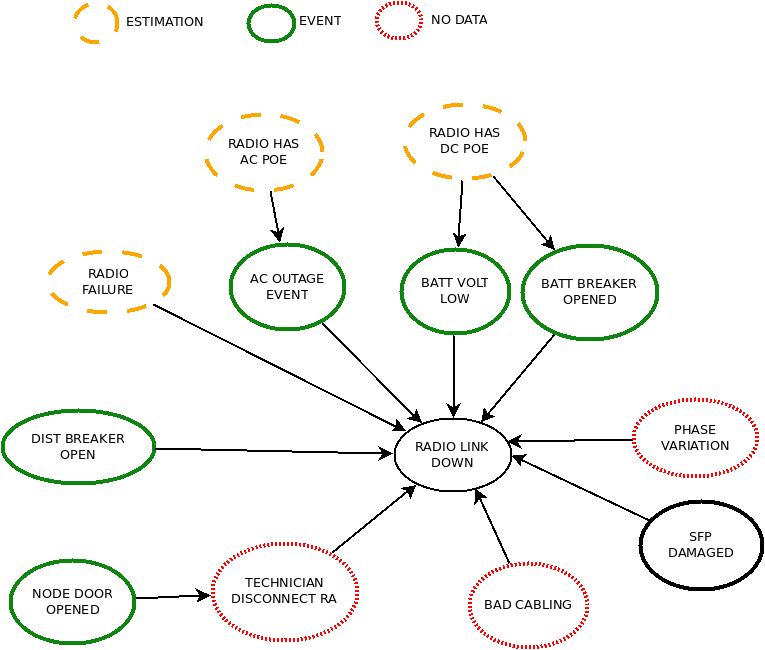
\includegraphics[scale=0.5]{LinkDownBBN.png}
  \centering
  \caption{\textit{A draft of the BBN for Link Down on a Radio}}
  \label{fig:LinkDownBBN}
\end{figure}	

\newpage
\section{Further Analysis}
Based on the previous analysis and one subsequent alarm exploration some further scenarios will be propose and some of them have been already tested.

Specifically, the following scenarios have been tested:

\begin{itemize}
\item Scenario 1 - DPS failure, Breaker Open, Low Battery Voltage + Link Down, Vendor 1: In this scenario $(a_t)$ is the union of the following alarms: DPS Failure, DistributionBreakerOpen, BatteryBreakerOpen and MajorLowBattVolt and $(a_i)$ is a LinkDown alarm in the L2 Switch.
\item Scenario 2 - Breaker Open, Low Batter Voltage + Link Down, Vendor 2: In this scenario $(a_t)$ is the union of the following alarms: BreakerOpen and Low Battery Voltage and $(a_i)$ is a LinkDown alarm in the L2 Switch.
\end{itemize}

The results are summarised in the following table: 

\begin{center}
 \begin{tabular}{||c | c | c | c ||} 
 \hline\hline
 Scenario  & $P_t(a_t)$ & $P_t(a_i|a_t)$ \\ 
 \hline
 Scenario 1& 0.0059 & 0.718 \\  
 \hline
 Scenario 2 & 0.031 & 0.877 \\  

 \hline\hline
\end{tabular}
\end{center}

It can be seen from the results that now $a_t$ is a better predictor of $a_i$. The drawback is that $P(a_t)$ is low.
\\\\
There are other scenarios discovered but not tested yet. The following are the discovered scenarios for Vendor 2 Switch:

\begin{itemize}
\item When there is an Optical Transmitter Output Power Low alarm there is a Laser Bias Current Out of Range alarm and possibly a Link Down on a 10G port.
\item Then there is an Optical Receiver Power Low alarm there is a Loss of Continuity alarm and possibly a Link Down.
\item When there is a Link Aggregation Group partial loss of capacity there is a Link Down, a System not redundant alarm and possibly an Optical Receiver Low.
\item When there is a Link Aggregation Group partial loss of capacity there is an Unexpected Service OAM MEP Id alarm.
\end{itemize}
\end{document}
